\documentclass[11pt]{article}
\usepackage{amsmath,amssymb,amsfonts,epsfig,algorithm,algorithmic,url, mathtools, indentfirst, color, soul}

\textheight 8.8truein
\parskip 0.1in
\topmargin -0.5truein
\textwidth 6.5truein
\oddsidemargin -0.05in
\evensidemargin -0.05in
% \renewcommand{\baselinestretch}{1.2}   %line space adjusted here
\setcounter{footnote}{0}
\sloppy

\renewcommand{\theequation}{\thesection.\arabic{equation}}
\newcommand{\newsection}{\setcounter{equation}{0}\section}

% redefining commonly used symbols
\DeclareMathOperator{\trace}{Tr}

\newtheorem{theorem}{Theorem}
\newtheorem{proposition}[theorem]{Proposition}
\newtheorem{lemma}[theorem]{Lemma}
\newtheorem{corollary}[theorem]{Corollary}
\newtheorem{definition}[theorem]{Definition}

\begin{document}
\title{\bf EE394V Power System Operations and Control\\
Learning for DC-OPF: Classifying active sets using neural nets 
}
\date{\today}
\author{JeeHyun Park}
%\normalsize{}
\maketitle
\begin{abstract}
Optimal power flow is used in power system operational planning to estimate the most economical efficiency solution while satisfying demand and safety margins. Due to increasing uncertainty and variability in energy sources and demand, the optimal solution needs to be updated near real-time to respond to observed uncertainty realizations. However, the existing method of solving the optimal problem could not cope with frequent updating due to the high computational complexity. To address this issue, a method was proposed to learn the mapping between the uncertainty realization and the active constraints set at optimality. In this paper, we propose the use of neural networks as a classifier learning the mapping between the uncertainty realization and the active constraints set at optimality, which has an extremely low computational complexity. Through experiments, we demonstrate the remarkable performance of this approach and visualize clusters of constraints on systems in the IEEE PES PGLib-OPF benchmark library.
\end{abstract}



\section{Introduction}\label{sec:intro}
DC optimal power flow (OPF) is one of linear optimization problem to estimate the most economical efficiency solution. Also, the solution satisfies the constraints related to demand and safety. Due to increasing increasing integration of renewable, as well as complexity of demand-side behavior, estimating the solution of DC optimal flow needs to be updated near real-time in response to observed uncertainty realization. Traditionally, affine control policy is proposed to address frequent updating issue. This method allows re-solving the OPF at a much faster time scale. However, due to its high computational complexity, it has limitations for tight latency requirements and large size of systems. In this paper, we propose the use of neural network as a classifier to enable extremely low computational complexity compared to the traditional method. Moreover, to boost up the performance, the classifier will learn the mapping from uncertainty realization $\omega$ to active constraints set $\mathcal{A^{\star}}$ at optimality instead of directly map to the adjustment in generation.



\section{Problem Formulation}\label{sec:problem}
\subsection{OPF Problem for a Given Uncertainty Realization}
According to \cite{1802.09639}, we could assume the system has $n$ generators, $m$ transmission lines, $v$ buses, and $v$ loads. We set a graph $\mathcal{G}( \mathcal{V}, \mathcal{E})$, where $\mathcal{V}$ denotes the nodes of the graph corresponding to the buses with $\left| \mathcal{V} \right| = v$, and the edges $\mathcal{E}$ denote the transmission lines with $\left| \mathcal{E} \right| = m$.

\subsubsection{Control Policy}
A $control \; policy \; \rho : \Omega \rightarrow \mathbb{R}^{n}$ is a mapping that adjusts the generation in response to uncertainty realization $\omega \in \Omega$. 

\begin{align}\label{eq:opf}
\rho^{\star}\left (  \omega \right )\in \underset{p}{\mathrm{argmin}} \; c^{\top }p \\
\textrm{s.t.} ~ &~ e^{\top }p=e^{\top }\left ( d -\omega  \right ) \\
~&~ p^{min}\leq p\leq p^{max} \\
~&~ f^{min}\leq M\left ( Hp +\omega -d \right )  \leq f^{max}
\end{align}

\subsubsection{Feasible Set of Polyhedral Constraints}
\begin{align}\label{eq:opf_poly}
\mathcal{P}\left ( \omega \right ) =  \{ p\in\mathbb{R}^{n}:
~ &~p^{min}\leq p\leq p^{max}, \nonumber \\
~ &~ f^{min}\leq M\left ( Hp +\omega -d \right )  \leq f^{max}, \nonumber \\
~ &~ e^{\top }p=e^{\top }\left ( d -\omega  \right )  \}
\end{align}

In the following analysis, we constrict ourselves to the set $\Omega^{R}\coloneqq\left \{ \omega:\mathcal{P}^{\star} \left ( \omega \right )\neq \emptyset \right \}$ of recovery scenarios, i.e., the scenario for which a feasible solution can be found. 

\subsubsection{Affine Control Policy}
\begin{align}\label{eq:opf_poly_compact}
\mathcal{P}\left ( \omega \right ) =  \{ p:
~ &~ Ap\leq b+C\omega, \; e^{\top }p=e^{\top }\left ( d -\omega  \right )  \}, \\
\text{where}
~ &~ A=\begin{bmatrix}I\\ -I\\ MH\\ -MH\end{bmatrix} \in \mathbb{R}^{2\left(n+m\right)\times n},
~ &~ C=\begin{bmatrix}0\\ -0\\ M\\ -M\end{bmatrix} \in \mathbb{R}^{2\left(n+m\right)\times v}, \nonumber \\
~ &~ b=\begin{bmatrix}p^{max}\\ -p^{min}\\ f^{max}+Md\\ -f^{min}+Md\end{bmatrix} \in \mathbb{R}^{2\left(n+m\right)}. \nonumber
\end{align}

\begin{align}\label{eq:opf_affine}
p^{\star}=B^{-1}\begin{bmatrix}
b_{\mathcal{A}}+C_{\mathcal{A}}\omega\\ 
e^{\top}\left(d-\omega\right)
\end{bmatrix} \coloneqq\rho^{\mathcal{A}}\left(\omega\right) \\
\text{where}
~ &~ B=\begin{bmatrix} A_{\mathcal{A}}\\ e^{\top} \end{bmatrix} \nonumber \\
~ &~ \mathcal{A} = \left \{ i_{1}, i_{1}, ..., i_{n-1} \right \}, \nonumber \\
~ &~ A_{\mathcal{A}} \coloneqq \text{the sub-matrix of } A \text{ formed by row in } \mathcal{A}, \nonumber \\
~ &~ b_{\mathcal{A}} \coloneqq \text{the sub-vector of } b \text{ formed by row in } \mathcal{A}, \nonumber \\
~ &~ C_{\mathcal{A}} \coloneqq \text{the sub-matrix of } C \text{ formed by row in } \mathcal{A}. \nonumber
\end{align}

\subsubsection{Ensemble Control Policy}
\begin{align}\label{eq:opf_predict}
\hat{\rho}\left(\omega\right) & \coloneqq \underset{\rho^{\mathcal{A}}\left(\omega\right):\mathcal{A}\in I}{\mathrm{argmin}} \; c^{\top}\rho^{\mathcal{A}}\left(\omega\right) \\
\textrm{s.t.} 
~ &~ \rho^{\mathcal{A}}\left(\omega\right) \in \mathcal{P}\left(\omega\right) \nonumber \\
& \text{where } I \text{ is the set of important active sets.} \nonumber
\end{align}

\subsubsection{Learning Optimal Solutions by Classification of Active Sets}
\begin{figure}[h]\label{fig:opf_nns}
\centering
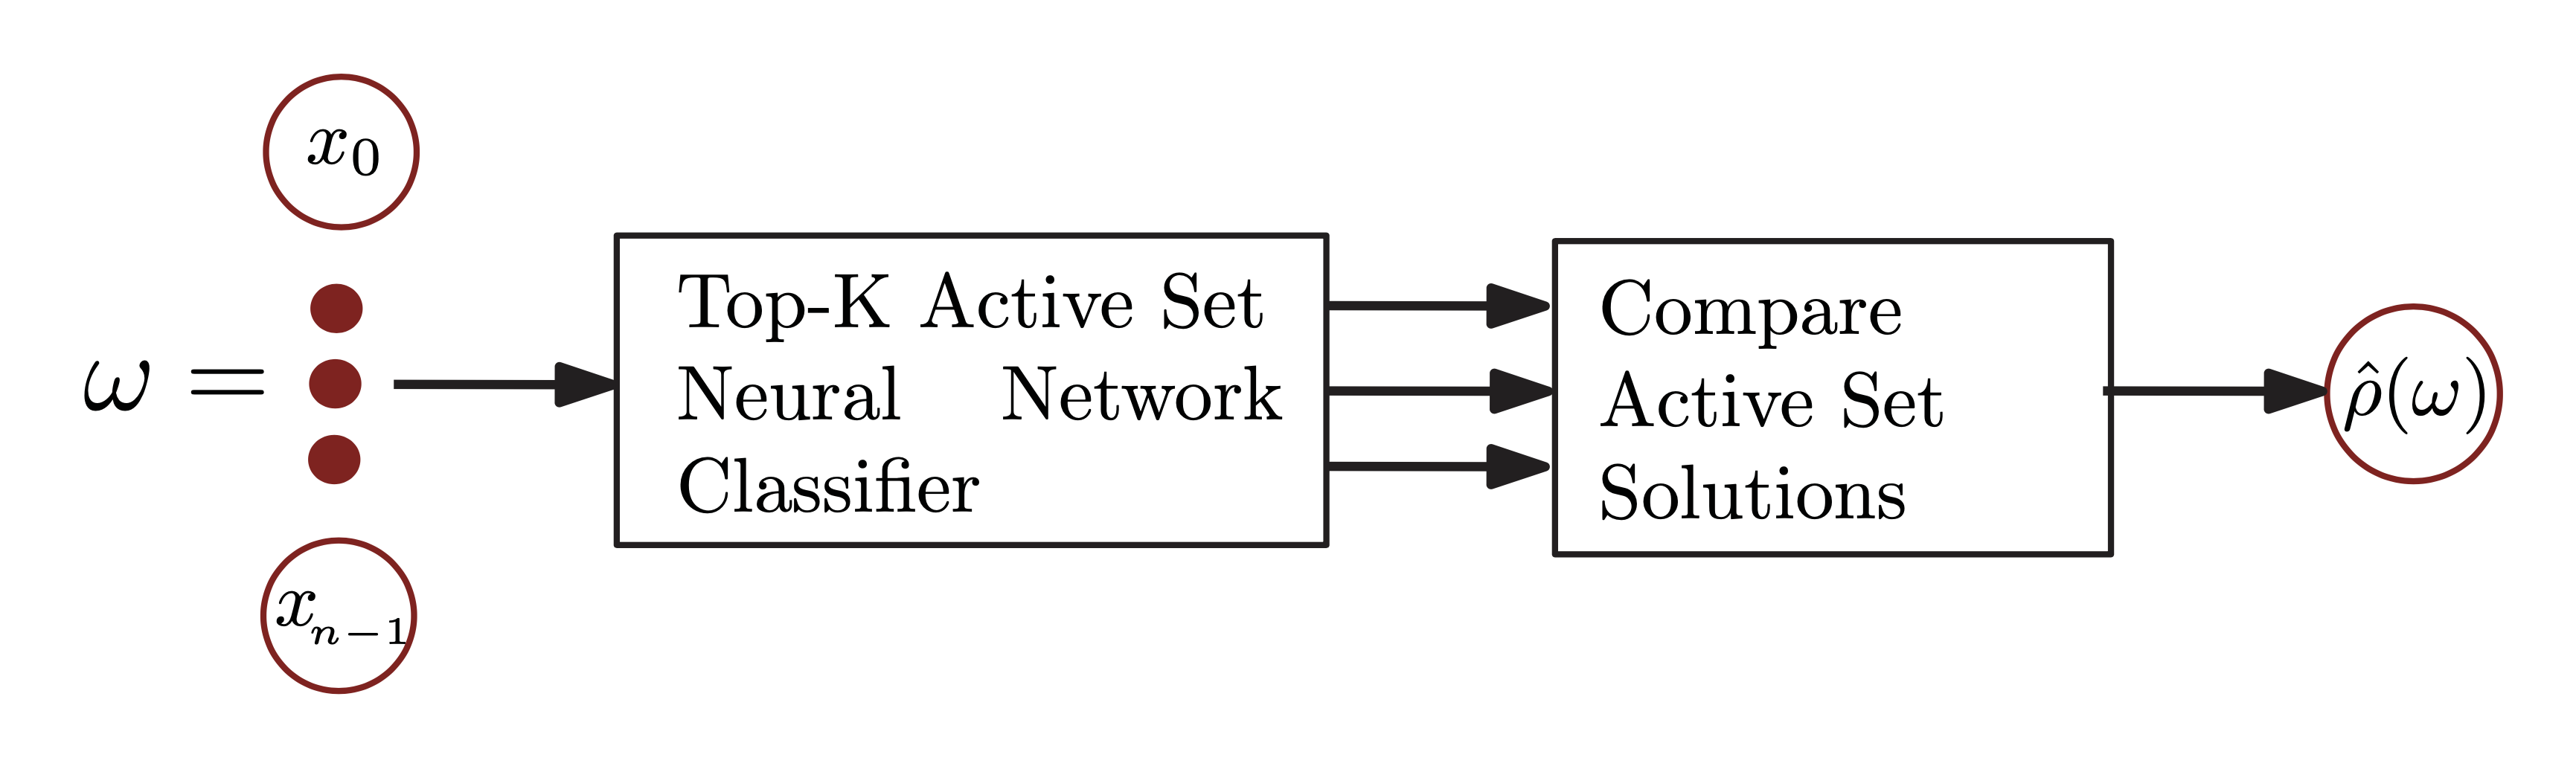
\includegraphics[scale=0.2]{report/figure/OPF NNs Classifier.png}
\caption{OPF Solution via Neural Network Classifier. \cite{10.1109/ptc.2019.8810819}}
\end{figure}
We employ the classification algorithm to learn the mapping from uncertainty realization $\omega$ to the corresponding active constraint set $\mathcal{A}^{\star}\left( \omega \right)$. We use neural network to build a classifier $\hat{\rho}$, the details are described in 2.2. The followings are metrics of the performance of the classifier.

\begin{align}\label{eq:acc}
\eta_{single} = \mathbb{P}_{\omega}\left(\hat{\mathcal{A}} \left(\omega \right)=\mathcal{A}^{\star}\left(\omega \right) \right) \\
\eta_{topK} = \mathbb{P}_{\omega}\left(\hat{I}_{K} \left(\omega \right) \ni \mathcal{A}^{\star}\left(\omega \right) \right)
\end{align}

\subsection{Classification}
\begin{figure}[h]\label{fig:nns_arch}
\centering
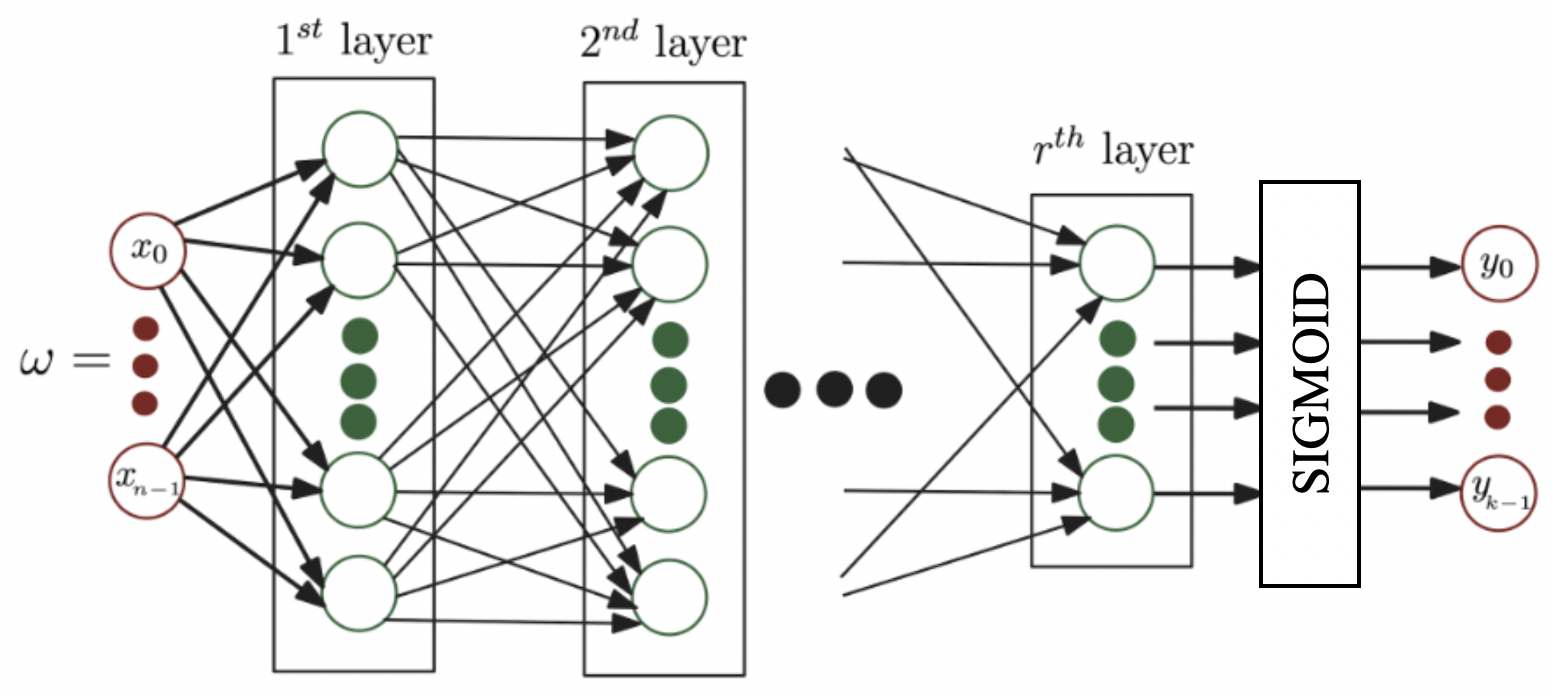
\includegraphics[scale=0.31]{report/figure/NNs_arch.png}
\caption{Architecture of the Neural Network Classifier.}
\end{figure}
\subsubsection{Neural Network Classifier}


This section will cover the architecture of neural network as a classifier. Also, we will specify the input and output data for the classifier. We will use Tensorflow or Pytorch for the experiments. 

This section will cover training process such as how to improve performance by adjusting the hyper-parameters and implementing batch normalization and drop-out.



\section{Numerical Experiments}\label{sec:tests}
\subsection{Dataset:  IEEE PES PGLib-OPF Benchmark Library}
This section will cover the analysis and pre-processing of the dataset \cite{pglib-opf}. 

\subsection{Experiments Rsults}
This section will cover the results for the following experiments.
\begin{itemize}
  \item Set up OPF Test-cases for the learning
  \item Check probability distribution of active sets of different OPF test-cases
  \item Observation of the change of accuracy according to the number of layers of fully connected layer (FCN).
  \item Check accuracy of active set top-K classification for different test cases with change in training data set size.
\end{itemize}



\section{Conclusions and Futureworks }\label{sec:conclusions}


In this section, we will discuss whether the performance of classification is satisfactory and whether online updating is possible due to the reduced computational complexity. As further studies, we will discuss \hl{how to extend the proposed method to AC OPF with non-linear variations}. Also, we will discuss about \hl{setting a set of parallel binary classifiers to predict the status of individual constraints separately, which will be an approach to develop a deeper understanding of various operational patterns, such as clustering of constraints.} 

\begin{thebibliography} {TL99}
\bibitem{learning_dc_opf} 
{\sc D. Deka and S. Misra,} 
"Learning for DC-OPF: Classifying active sets using neural nets," 2019 IEEE Milan PowerTech, Milan, Italy, 2019, pp. 1-6, doi: 10.1109/PTC.2019.8810819.

\bibitem{}
{\sc R. D. Christie, B. F. Wollenberg and I. Wangensteen,} 
"Transmission management in the deregulated environment," in Proceedings of the IEEE, vol. 88, no. 2, pp. 170-195, Feb. 2000, doi: 10.1109/5.823997.

\bibitem{statistical_learning}
{\sc Y. Ng, S. Misra, L. A. Roald and S. Backhaus,} 
"Statistical Learning for DC Optimal Power Flow," 2018 Power Systems Computation Conference (PSCC), Dublin, 2018, pp. 1-7, doi: 10.23919/PSCC.2018.8442859.

\bibitem{learing_constrained_op}
{\sc Misra, Roald, and Yeesian,} 
“Learning for Constrained Optimization: Identifying Optimal Active Constraint Sets,” arXiv.org, 16-Jan-2019. [Online]. Available: https://arxiv.org/abs/1802.09639. [Accessed: 10-May-2020].



\bibitem{batch_norm}
{\sc Sergey, }
“Batch Normalization: Accelerating Deep Network Training by Reducing Internal Covariate Shift,” arXiv.org, 02-Mar-2015. [Online]. Available: https://arxiv.org/abs/1502.03167. [Accessed: 10-May-2020].

\bibitem{dropout}
{\sc N. Srivastava, G. Hinton, A. Krizhevsky, I. Sutskever, and R. Salakhutdinov,} 
“Dropout: A Simple Way to Prevent Neural Networks from Overfitting,” Journal of Machine Learning Research, 01-Jan-1970. [Online]. Available: http://jmlr.org/papers/v15/srivastava14a.html. [Accessed: 10-May-2020].

\bibitem{bin_cross_entropy}
{\sc }
“Binary crossentropy loss function: Peltarion Platform,” Peltarion.com. [Online]. Available: https://peltarion.com/knowledge-center/documentation/modeling-view/build-an-ai-model/loss-functions/binary-crossentropy. [Accessed: 05-May-2020]

\bibitem{adam}
{\sc Kingma, D. P., Jimmy, and Ba,} 
“Adam: A Method for Stochastic Optimization,” arXiv.org, 30-Jan-2017. [Online]. Available: https://arxiv.org/abs/1412.6980. [Accessed: 10-May-2020].

\bibitem{pglib-opf}
Power-Grid-Lib, “power-grid-lib/pglib-opf,” GitHub, 03-Sep-2019. [Online]. Available: https://github.com/power-grid-lib/pglib-opf. [Accessed: 10-May-2020].

\bibitem{transformer}
{\sc Vaswani, Ashish, Shazeer, Noam, Parmar, Niki, Jakob, Jones, Gomez, A. N., Kaiser, Lukasz, Polosukhin, and Illia,}  
“Attention Is All You Need,” arXiv.org, 06-Dec-2017. [Online]. Available: https://arxiv.org/abs/1706.03762. [Accessed: 10-May-2020].

\bibitem{}
{\sc }

\bibitem{1802.09639}
Sidhant Misra, Line Roald and Yeesian Ng.
\newblock “Learning for Constrained Optimization: Identifying Optimal Active Constraint Sets,” 2018;
\newblock arXiv:1802.09639.

\bibitem{}
{\sc D. Walkup and R. Wets,}
“Lifting projections of convex polyhedra,” Pacific Journal of Mathematics, vol. 28, no. 2, pp. 465–475, 1969.


\end{thebibliography}

\end{document}
